\subsection{Passarela sobre a ravina de Ovejas, Espanha}

A passarela sobre a ravina de Ovejas, província de Alicante, Espanha é uma passarela de 45 metros (\autoref{ovejas} e \autoref{ovejas-2}), protendida, feita com treliças do tipo Warren de CUAD (\autoref{ovejas-long} e \autoref{ovejas-bottom}). Foi a primeira passarela feita completamente com treliças de CUAD. A espessura do tabuleiro é de apenas 3 cm e a resistência do concreto é de 150 MPa. A \autoref{ovejas-section} e a \autoref{ovejas-section-2} mostram a configuração  da passarela com mais detalhes.

\begin{figure}[htb]
	\caption{\label{ovejas}Passarela sobre a ravina de Ovejas, Província de Alicante, Espanha.}
	\begin{center}
	    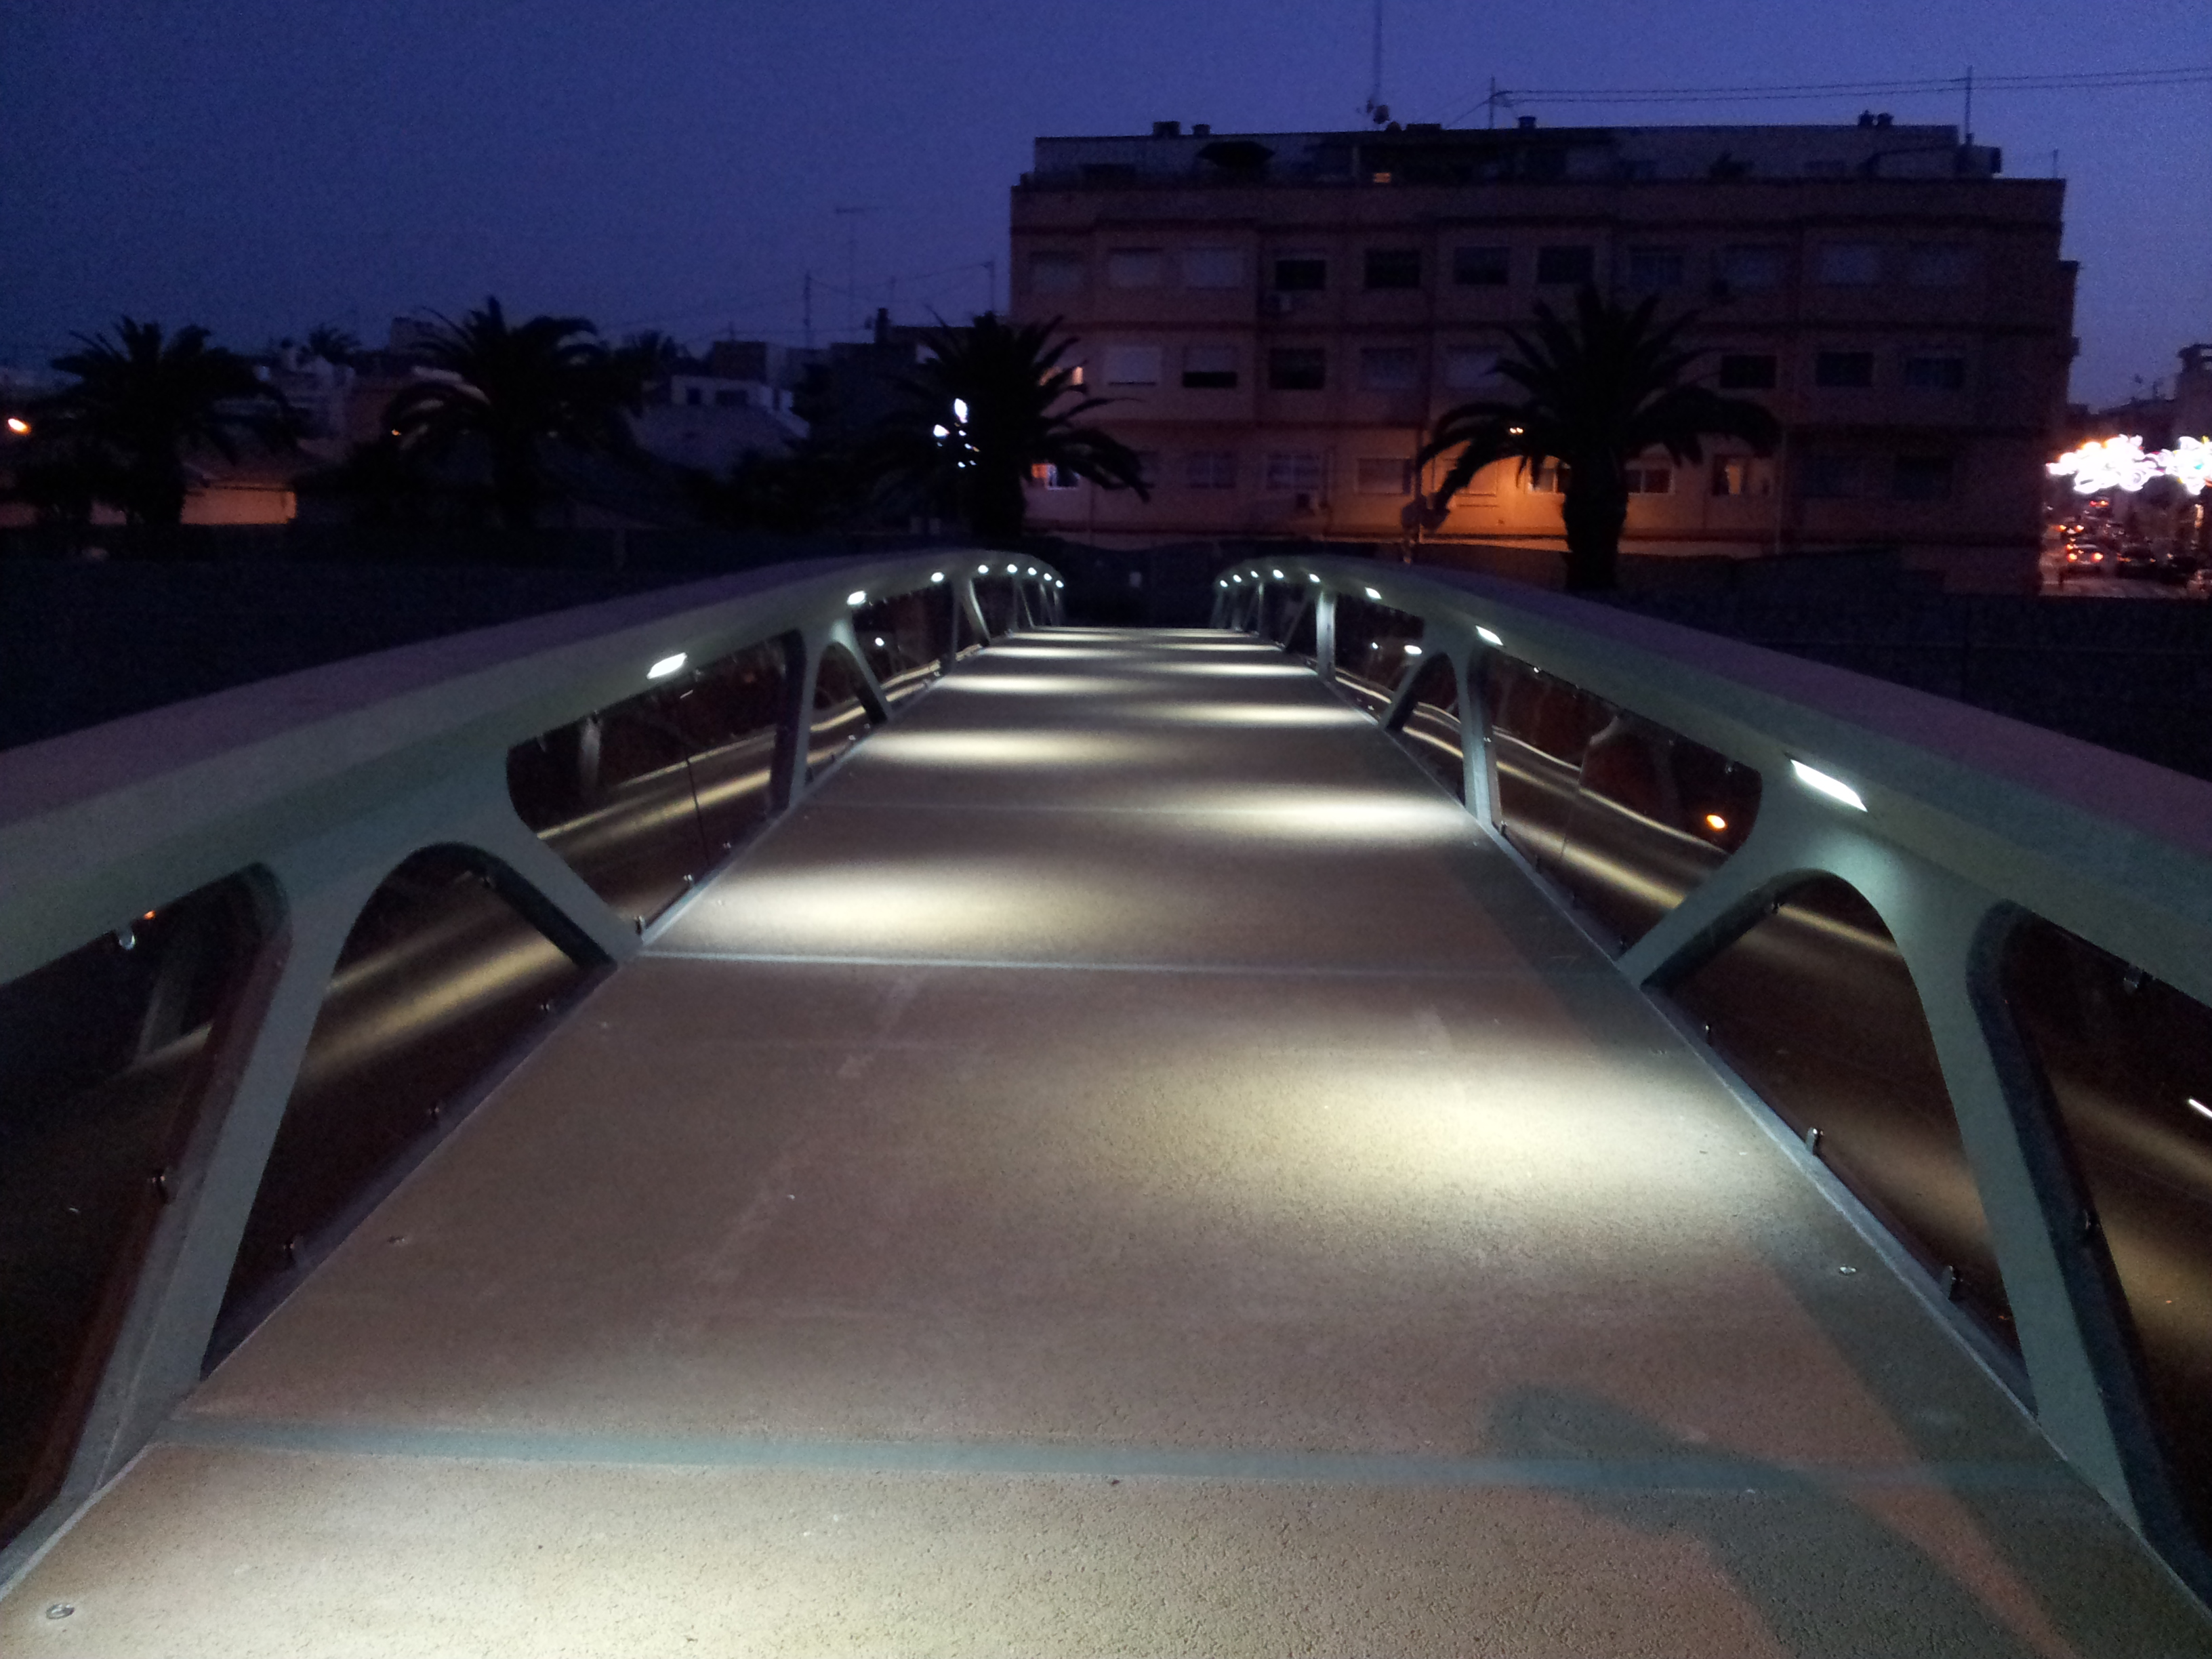
\includegraphics[max width=\textwidth]{passarela-ovejas.jpg}
	\end{center}
	\fonte{\citeonline{RDC}}
\end{figure}

\begin{figure}[htb]
	\caption{\label{ovejas-2}Representação gráfica da passarela de Ovejas.}
	\begin{center}
	    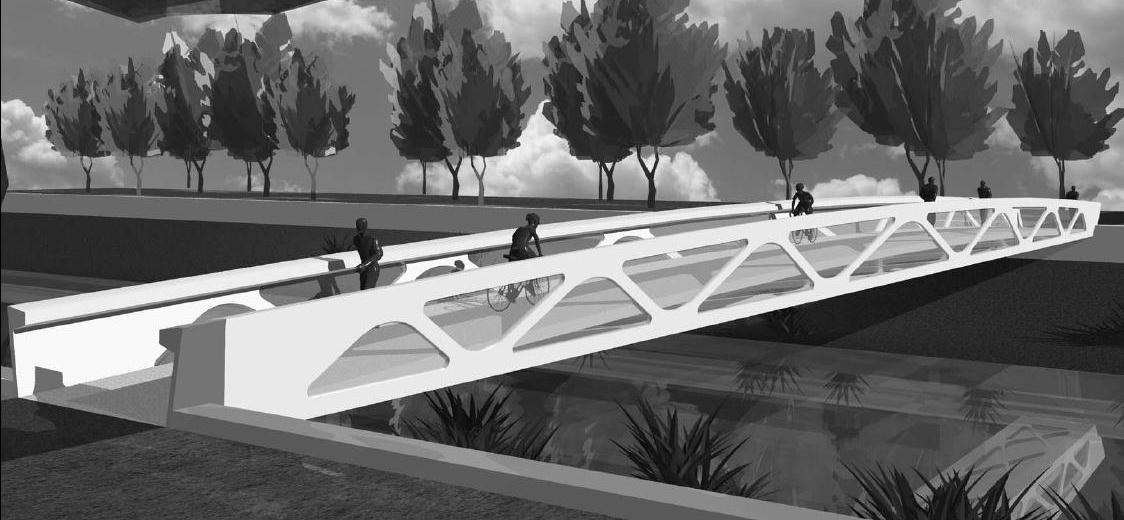
\includegraphics[max width=\textwidth]{ovejas-overview.png}
	\end{center}
	\fonte{\citeonline{Lopez}}
\end{figure}

\begin{figure}[htb]
	\caption{\label{ovejas-long}Vista longitudinal da passarela.}
	\begin{center}
	    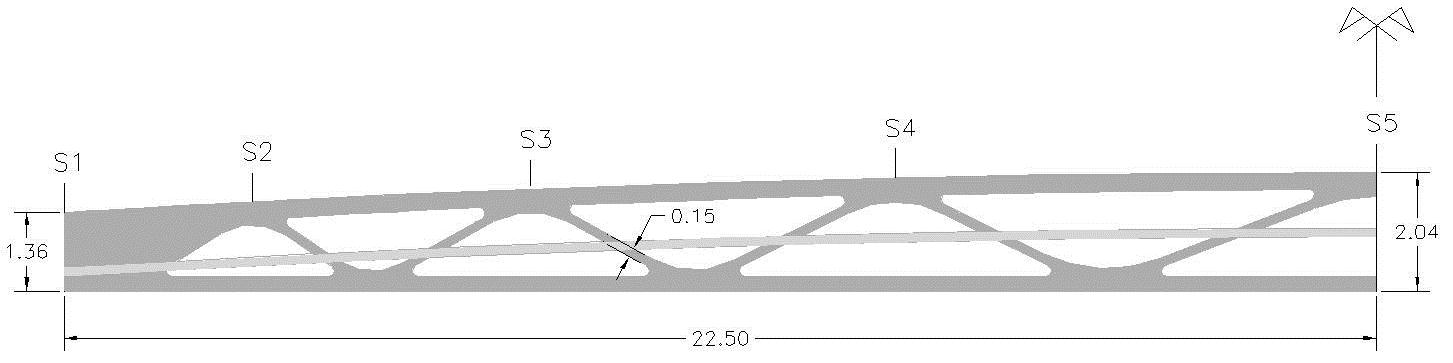
\includegraphics[max width=\textwidth]{ovejas-longitudinal.png}
	\end{center}
	\fonte{\citeonline{Lopez}}
\end{figure}

\begin{figure}[htb]
	\caption{\label{ovejas-bottom}Treliças abaixo do tabuleiro.}
	\begin{center}
	    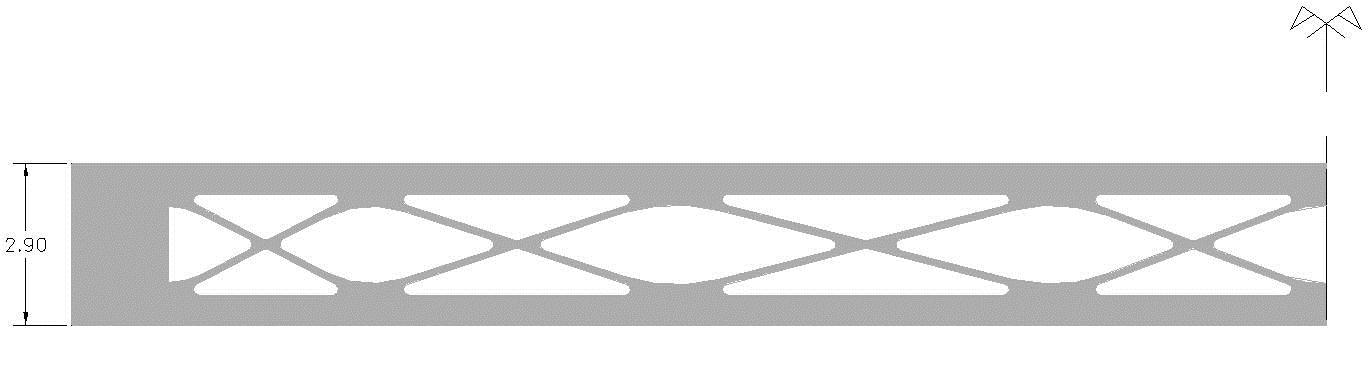
\includegraphics[max width=\textwidth]{ovejas-bottom.png}
	\end{center}
	\fonte{\citeonline{Lopez}}
\end{figure}

\begin{figure}[htb]
	\caption{\label{ovejas-section} Corte transversal da passarela com detalhamento.}
	\begin{center}
	    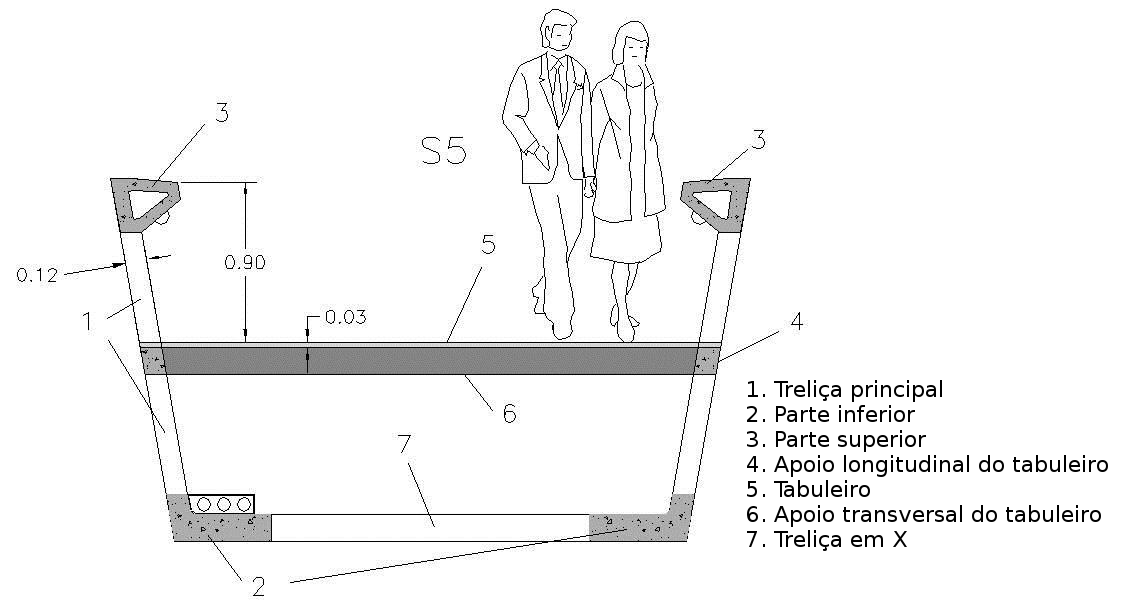
\includegraphics[max width=\textwidth]{ovejas-corte.png}
	\end{center}
	\fonte{\citeonline{Lopez}}
\end{figure}

\begin{figure}[htb]
	\caption{\label{ovejas-section-2}Corte transversal da passarela com detalhamento.}
	\begin{center}
	    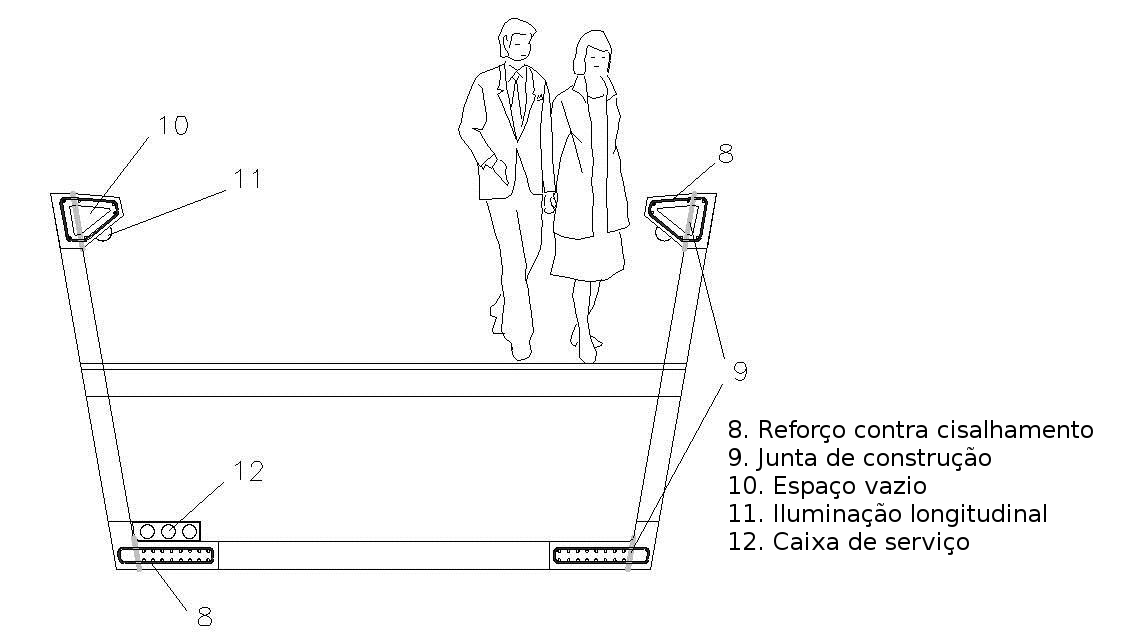
\includegraphics[max width=\textwidth]{ovejas-corte2.png}
	\end{center}
	\fonte{\citeonline{Lopez}}
\end{figure}

A passarela foi moldada na fábrica e transportada por inteiro para sua locação final. O estudo do carregamento da estrutura foi feito com o software SAP2000, considerando as ações especificadas na \autoref{ovejas-acoes}. O traço de concreto utilizado é mostrado na \autoref{ovejas-traco}.


\begin{table}[htb]
	\IBGEtab{%
		\caption{Ações consideradas no projeto da passarela.}
		\label{ovejas-acoes}
		}{%
		\begin{tabulary}{\linewidth}{CC}
			\toprule
			Propriedade                                    & Valor \\
			\midrule \midrule
			Peso próprio                                   & 4,3 kN/m\textsuperscript{2} \\ \midrule
			Carregamento dinâmico característico	       & 5,0 kN/m\textsuperscript{2} \\ \midrule
			Carregamento dinâmico frequente                & 2,0 kN/m\textsuperscript{2} \\ \midrule
			Deformação vertical sob carregamento frequente & 3,6 cm                      \\ \midrule
			Velocidade básica do vento	                   & 18 m/s                      \\ \midrule
			Temperatura mais alta	                       & 34,2\textsuperscript{\degree}C   \\ \midrule
			Temperatura mais baixa                         & 11,5\textsuperscript{\degree}C    \\ \midrule 
			Aceleração sísmica máxima horizontal/vertical  & 3,44/2,41 m/s\textsuperscript{2} \\
			\bottomrule
		\end{tabulary}%
	}{%
	\fonte{\citeonline[p.~899]{Lopez}.}%
			%\nota{Esta é uma nota, que diz que os dados são baseados na regressão linear.}
			%\nota[Anotações]{Uma anotação adicional, que pode ser seguida de várias outras.}
	}
\end{table}

\begin{table}[htb]
	\IBGEtab{%
		\caption{Traço do CUAD utilizado.}
		\label{ovejas-traco}
	}{%
	\begin{tabulary}{\linewidth}{CC}
		\toprule
		Material                                       & Quantidade (kg/m\textsuperscript{3}) \\
		\midrule \midrule
		Cimento (a/c = 0,213)                          & 1000 \\ \midrule
		Fumo de sílica                 	               & 150  \\ \midrule
		Areia 0,5 mm                                   & 702  \\ \midrule
		Areia 1,8 mm                                   & 380  \\ \midrule
		Água                  	                       & 213  \\ \midrule
		Superplastificante \textsuperscript{1}          & 9,06 \\ \midrule
		Fibras OL13/0.16 \textsuperscript{2}            & 78,1 \\ \midrule 
		Fibres RC80/40 BP \textsuperscript{2}           & 78,1 \\
		\bottomrule
	\end{tabulary}%
}{%
\fonte{\citeonline[p.~899]{Lopez}.}%
\nota{\textsuperscript{1)} Fração sólida de superplastificante;}
\nota{\textsuperscript{2)} 1\% em volume de cada fibra de Bekaert.}
%\nota[Anotações]{Uma anotação adicional, que pode ser seguida de várias outras.}
}
\end{table}